\documentclass{beamer}
\usetheme{metropolis}
\usepackage[font=footnotesize, labelfont=footnotesize]{caption}
\usepackage{graphicx}

\graphicspath{ {images/} }


\title{Introduction}
\subtitle{Wireless Mobile Software Engineering}
\date{28 February 2017}
\author{Steven "Steven"}
\institute{BINUS INTERNATIONAL}


\begin{document}
  \maketitle
  
  \begin{frame}{Some basic rules}
  	\begin{itemize}
		\item Phone should be silent at all time
		\item Laptop is fine
		\item Late policy
		\item All slides and handouts are available at github (goo.gl/Lb2VQQ) (Corrections to them are encouraged)
		\item All materials are sourced from https://developer.android.com/guide/index.html
	\end{itemize}
  \end{frame}
 
  
    \begin{frame}{Today's agenda}
     \begin{itemize}
        \item News
        \item Brief tour of Android platform stack
    	\item Android application fundamentals
        \item Application components
		\item Activity
		
	\end{itemize}
  \end{frame}
  
  \begin{frame}{News}
    \begin{center}
        News!
    \end{center}
\end{frame}
  
  \begin{frame}{Android platform stack - Lower level}
    \begin{center}
        \begin{figure}
            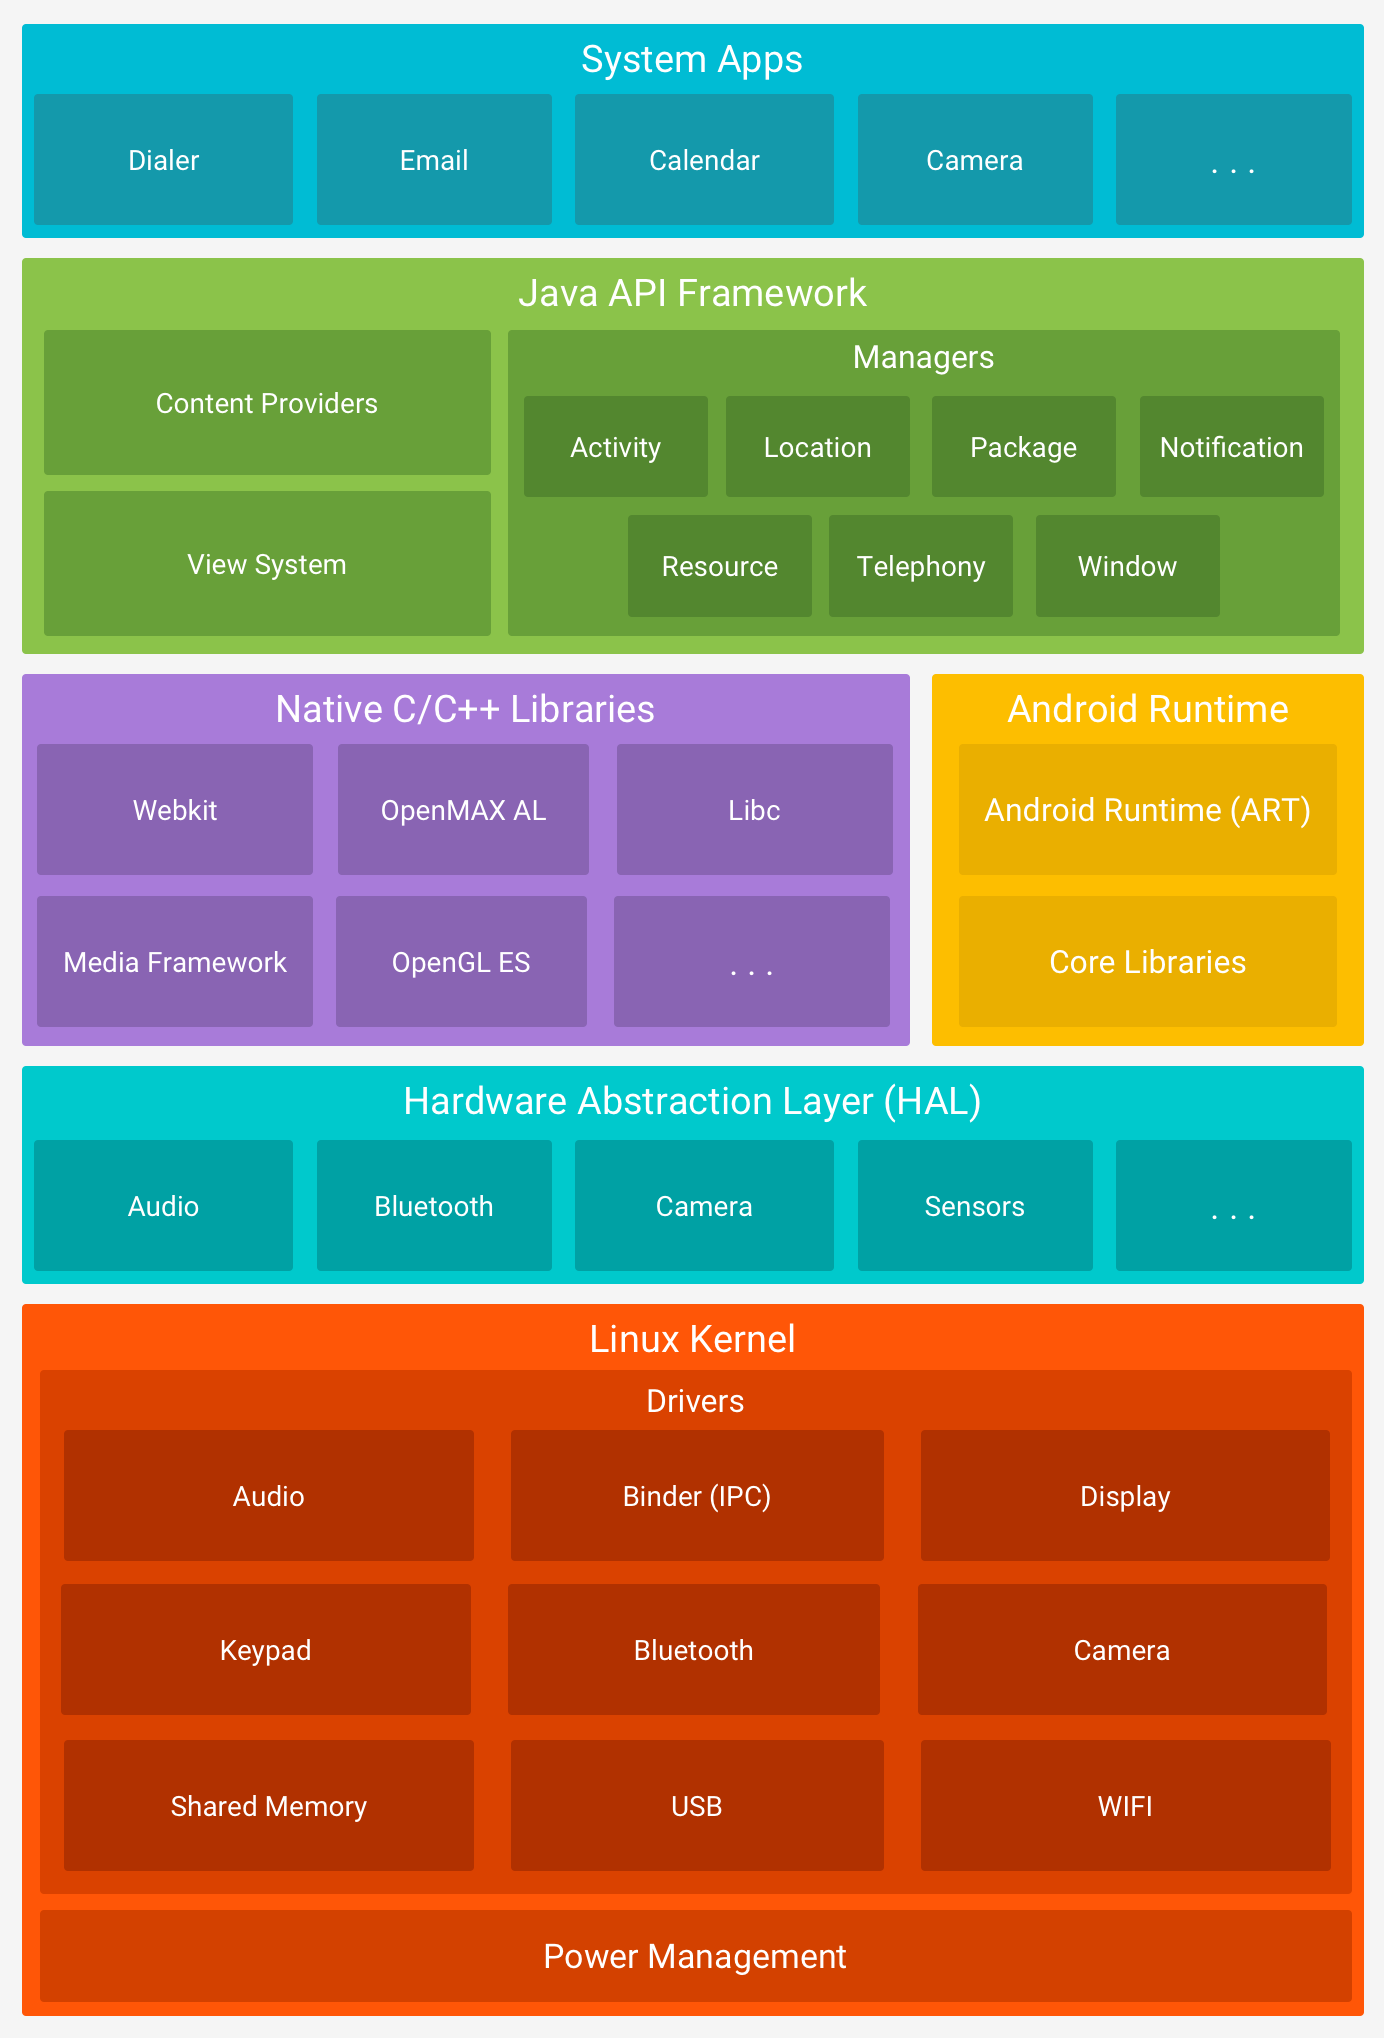
\includegraphics[clip, trim=0 0 0 37cm, width=.8\paperwidth]{android-stack}
            \caption{https://developer.android.com/guide/platform/index.html}
        \end{figure}
    \end{center}
\end{frame}

  \begin{frame}{Android platform stack - Higher level}
    \begin{center}
        \begin{figure}
            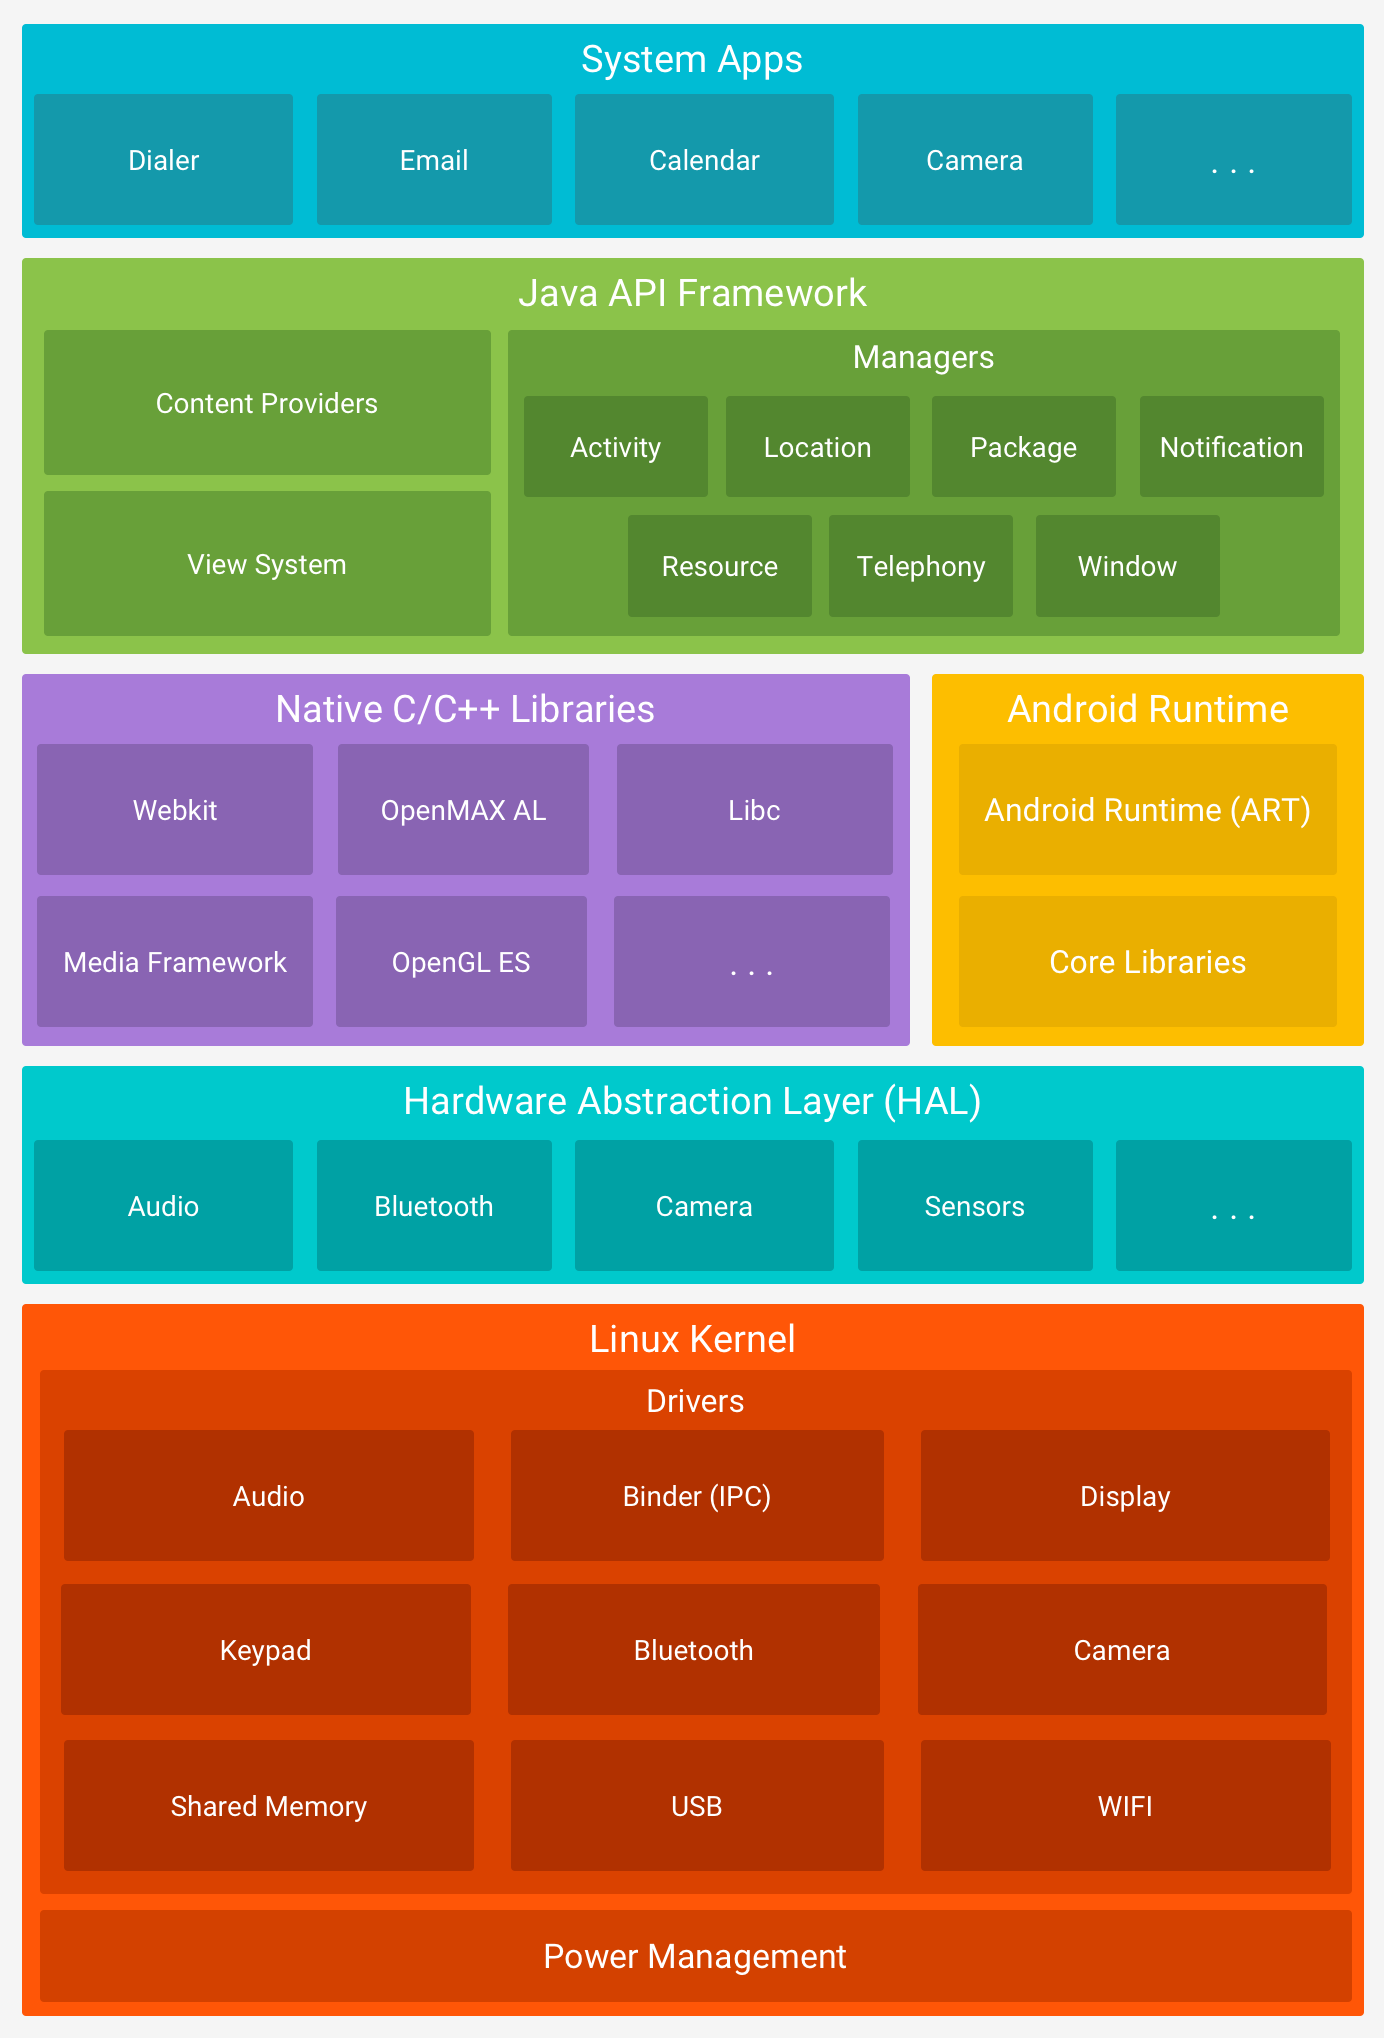
\includegraphics[clip, trim=0 36cm 0 0, width=.8\paperwidth]{android-stack}
            \caption{https://developer.android.com/guide/platform/index.html}
        \end{figure}
    \end{center}
\end{frame}

    \begin{frame}{Android platform stack - recap}
    \begin{center}
        \begin{figure}
            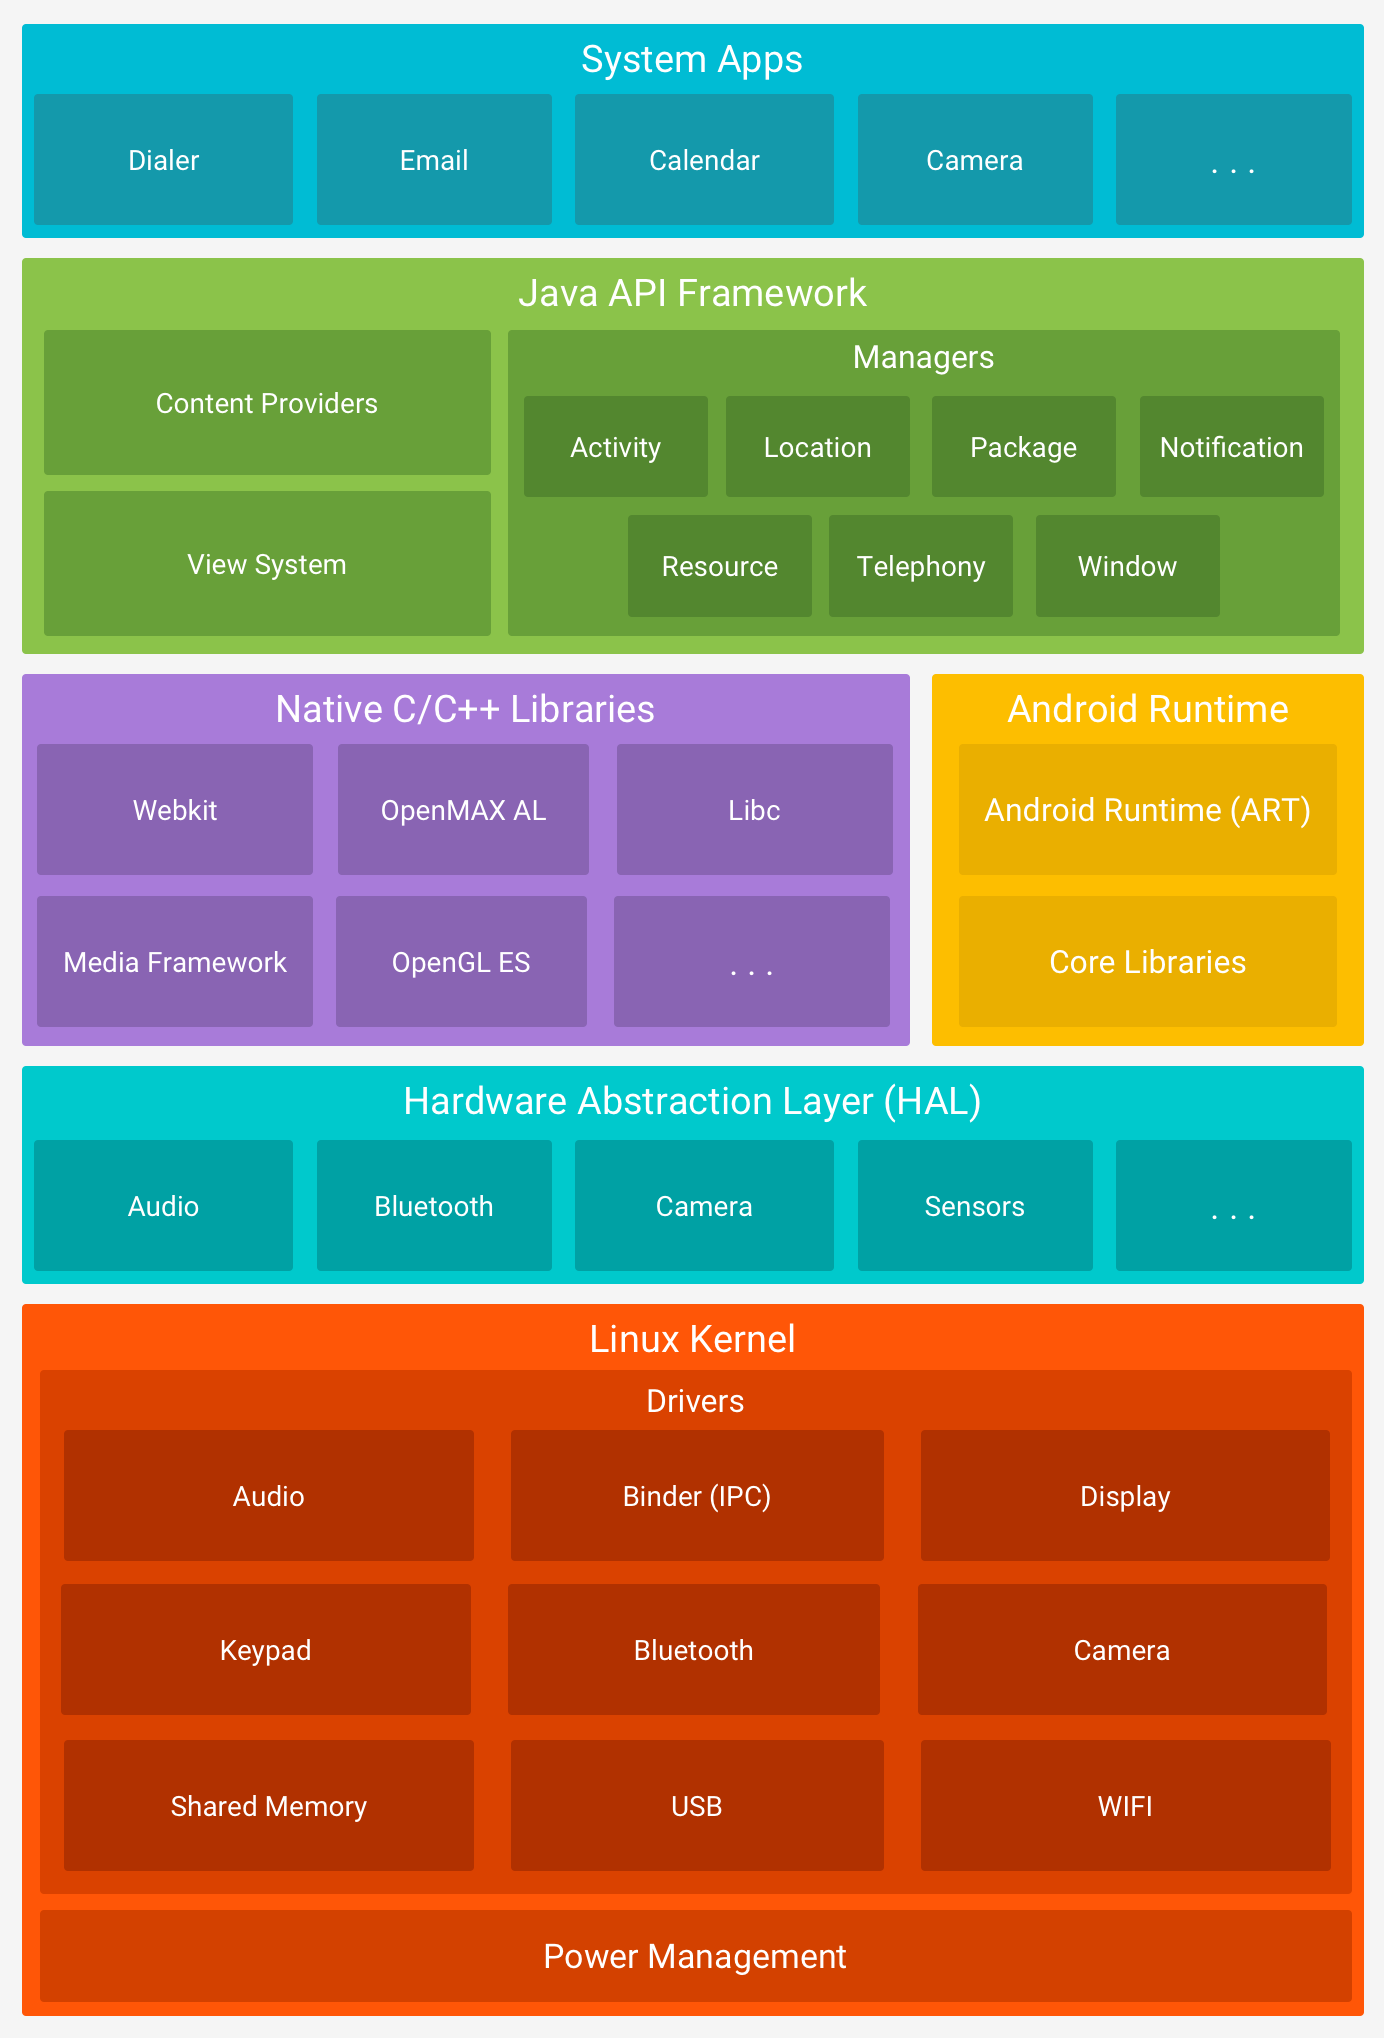
\includegraphics[scale=.1]{android-stack}
            \caption{Overview of the platform architecture}
        \end{figure}
    \end{center}
\end{frame}
  
    \begin{frame}{Android application fundamentals in a nutshell}
     \begin{itemize}

    	\item Android OS is basically multi-user Linux system
    	\item Each process lives on its own VM with its own Linux ID
        \item Android studio, take all your resources and code, compile and then archive it into an Android Package (.apk)
        \item Dalvik Virtual Machine will run the application byte code(.dex)
	\end{itemize}
  \end{frame}
    
   \begin{frame}{Application components}
   
     Entry point for system / user to enter your application
     \begin{itemize}

    	\item \textbf{Activity}
    	\item Service
    	\item Content provider
    	\item Broadcast receivers
	\end{itemize}
  \end{frame}
  
  
     \begin{frame}{Activity}
   
     Entry point for \textbf{user interaction} with your application
     \begin{itemize}
        \item Java class that ineherits \textbf{\textit{android.app.Activity}} class 
    	\item Android OS will start the main activity you choose in the manifest file
    	\item Your application's activity will be available for other application when sending appropriate \textit{intent}

	\end{itemize}
  \end{frame}
  
\begin{frame}{Activity Lifecylce}
    \begin{center}
        \begin{figure}
            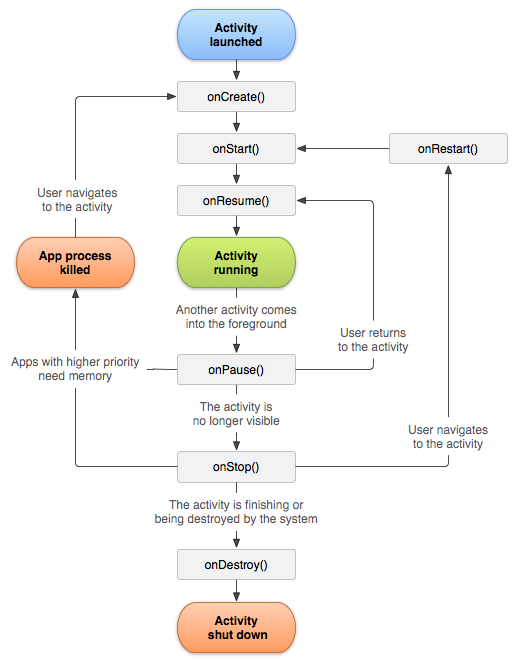
\includegraphics[scale=0.32]{activity_lifecycle}
            \caption{Activity lifecycle diagram [2]}
        \end{figure}
    \end{center}
\end{frame}


\begin{frame}{Live demo}
    \begin{center}
        Demo time
    \end{center}
\end{frame}
  
  
  \begin{frame}[fragile]{Lab today}
     \begin{itemize}
        \item Tutorial to create messaging app (Will use this theme throughout the class)
    	\item Check out your github repo, push your readme to your repo
    	\item \textbf{Reminder}: Final project phase 1 - 20\% \textbf{(21 March / in 3 weeks)}
	\end{itemize}
\end{frame}
\end{document}